\chapter{Requirement Specification}
\subsection{Introduction}
This chapter will describe the requirements needed for the multichannel audio/video playback system called Showman. This chapter contains an introductory overview of Showman in general that covers a System Description, System Overview and Usage Situation followed by Functional and Non-Functional Requirements. The chapter ends with a MoSCoW- and FURPS-analysis to organize a list of priorities needed to develop a functional prototype. \newline

\subsection{System Description}

The purpose of Showman is to play back prerecorded audio- and video-material during a concert performance. Prerecorded audio- and video-playback material  is colloquially called 'backing tracks'. The primary reason of backing track usage is to enhance a concert performance by play back additional material that artists on stage do not have the option or time to play themselves. \newline

User (or artist) uploads synchronized audio files in 44.1 kHz 16-bit .WAV-format and video files in MPEG-4 format to Showman before using Showman during showtime. User creates, edits and organizes playlist with a software application Graphical User Interface (GUI) on laptop (PC or Mac). The content of the playlist is the backing track material that user produced beforehand. After playlist creation, user uploads the playlist via a USB-connection to Showman's internal memory. \newline

Showman play back 8-tracks of audio along with video-content. The audio tracks can be connected directly into the XLR-inputs of a live sound mixer through Showman's XLR outputs, while the video-material can be connected to screens through Showman's HDMI-output.
User starts each song in the playlist separately by pressing the `Play'-button on Showman. The first song on the playlist begins and playback stops automatically (auto-stop) after each ending of a song. \newline

\begin{figure}[htb!]
\centering
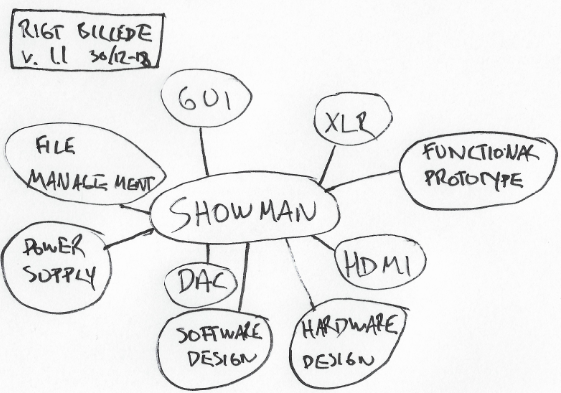
\includegraphics[scale=1]{./pictures/RigtBillede.png}
\caption{Content of Showman as a rich picture.}
\label{fig:RigtBillede.png}
\end{figure}

%\subsection{System Overview}

\subsection{Usage Situation} 

Showman's intended users are artists that utilize backing tracks at concert performances to enhance/augment their performance. Preconditions are essential to Showman, as user must have up to 4 stereo or 8 mono .WAV-files and a MPEG4-videofile available for each song that has backing tracks. The artist need to have produced the backing tracks beforehand. \newline

As Showman's intended usage conditions are tough touring conditions and periodic hard handling, Showman's user interface is a 2U 19'' rack mounted device with a LCD screen for user monitoring and panel buttons for navigation.   \newline

When the user have the necessary files available, the user assembles the playlist in the software application GUI and assigns the audio outputs. The GUI uploads the playlist project into specific folders in Showman's internal 500 GB flash memory. \newline

When user need to start playback of a song, all user need to do is press `Play' on the user panel. An auto-stop function after the end of each song in the project is embedded in Showman. \newline

\subsection{Actor-Context Diagram}

The figure below is an overview of actors that interact with Showman:

\begin{figure}[htb!]
\centering
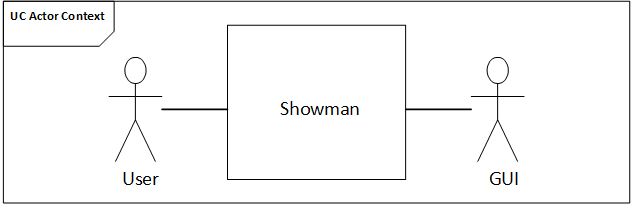
\includegraphics[scale=1]{./pictures/ActorContext.png}
\caption{Actor-Context diagram of Showman.}
\label{fig:ActorContext.png}
\end{figure}

\subsubsection{User}
User is the primary actor. User creates the playlist and uploads the playlist to Showman. User operates Showman. User's interaction with Showman is outlined in detail in the specification for the individual Use Cases. \newline

\subsubsection{GUI}
The Graphical User Interface (GUI) is the secondary actor. The GUI is the software application that handles the file management and playlist creation that is uploaded to Showman's interaction with Showman is outlined in detail in the specification for the individual Use Cases. \newline

\subsection{Functional Requirements}
This section presents the functional requirements outlined for Showman. The figure below presents a Use-Case diagram that displays the actors' relations to the Use-Cases followed by Fully Dressed Use-Cases. \newline

To keep this document brief and concise, only the first Use-Case is included. The additional Use-Cases will be explored further in the bachelor project.

%\subsubsection{Use-Case Diagram}

\subsubsection{Use-Case 1}

\begin{figure}[H]
\centering
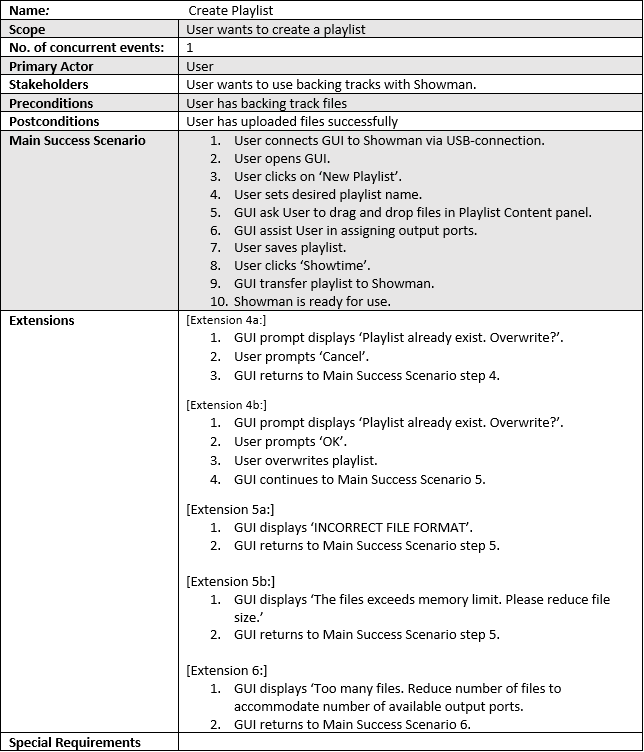
\includegraphics[scale=1]{./pictures/UC1.png}
\caption{Use-Case diagram of Use-Case 1.}
\label{fig:UC1.png}
\end{figure}

%\subsubsection{Use-Case 2}


%\subsubsection{Use-Case 3}


%\subsubsection{Use-Case 4}


%\subsubsection{Use-Case 5}


\subsection{Non-Functional Requirements}
Non-Functional Requirements (NFRs) are quality-demands, which are the qualities or constraints on the services of the functions offered by the system rather than a specific behaviour. Qualities are properties or characteristics of the system that its stakeholders care about and hence will affect their degree of satisfaction with the system. \\
Quality demands/NFRs should satisfy two attributes: \\
- Must be verifiable - e.g. measurable metrics.
- Should be objective. \newline

The NFRs are drawn up using two techniques: FURPS and MoSCoW to determine system requirements and to prioritize and rank Non-Functional Requirements. \\

\subsection{FURPS+}
FURPS+ is an acronym that represents a model classify a product's properties: \textbf{F}unctionality, \textbf{U}sability, \textbf{R}eliability, \textbf{P}erformance, \textbf{S}upportability and \textbf{+} (Design and Physical constraints, Interfaces, Legal, Test, Reuse, Economic constraints, Aesthetics, Comprehensibility, Techology tradeoff, etc.)  \newline

A point-system from 1-5 is used to classify priorities, where 1 is the lowest and 5 the highest priority. \\

\subsubsection{\textbf{F} - Functionality}
The functionality describes the capability (size and generality of feature set), reusability (combability, interoperability, portability) and security (safety and exploitability) of a system. \\

\textbf{Use-Case 1 - Create Playlist} \\
UC1 has the highest priority as it is essential for Showman to create playlists with GUI in order to operate Showman. \newline
\textbf{Score: 5} \\

\subsubsection{\textbf{U} - Usability} 
\textbf{Accessibility} \\
\textit{Description of the ease of access to system} \\
As the target group are touring artists and artist crew both with little to no time, the system need to be easy to use and operate with minimal learning curve. \newline
\textbf{Score: 4} \newline

\textbf{User Interface} \\
\textit{Description of the Graphical User Interface's functionality} \\
The system need a GUI that need minimal learning curve, and therefore has to be similar to GUIs of software applications such as ProTools, Apple Logic X, Ableton Live, Cymatic Audio uTool. \newline
\textbf{Score: 3}

\subsubsection{\textbf{R} - Reliability} 
\textbf{Predictability} \\
\textit{Description of the system's stability} \\
This requirement is ranked highly in order for User to be reliant on that filetransfer does not malfunction nor malfunction does not occur during operation of the system. \\
\textbf{Score: 4} \newline

\textbf{Maintainability} \\
\textit{Description of the system's maintainability} \\
This requirement is also ranked highly in order for User to be able to acquire spare parts in case something breaks as the system will be in transit daily and is exposed to hard handling or manufacturer/producer updates firmware or software application. \newline
\textbf{Score: 4} \newline

\subsubsection{\textbf{P} - Performance}
%The performance describes the speed, efficiency, resource consumption (power, RAM, cache, etc.), throughput, capacity, scalability of the system. \\
\textbf{GUI start-up time} \\
\textit{Description of the software application GUI's accessibility when opening software application} \\
Showman's GUI must be accessible max. 5 seconds after opening software application in order for User to create or edit a playlist and transfer playlist to Showman. \\
\textbf{Score: 3} \newline

\textbf{Showman start-up time} \\
\textit{Description of Showman's User Interface accessibility when turning Showman on} \\
Showman's UI must be available and accessible max. 5 seconds after turning the system on in order for User to play playlist. \newline
\textbf{Score: 3} \newline

\textbf{Execution time - File transfer} \\
\textit{Description of the fast the system can complete the given functionality described in the Use Cases} \\
This property is not ranked highly, as long as the file transfer is finished within a few minutes. A research in file transfer speed is needed to determine file transfer speed. \\
\textbf{Score: 2} \newline

\textbf{Execution time - Play playlist} \\
\textit{Description of how fast the system can complete the given functionality described in the Use Cases} \\
This property is ranked in the middle. Showman must start playback within ~ 5-10 microseconds of User pushing `Play'-button. A research in push buttons is needed to implement and determine speed of play playlist execution time. \\
\textbf{Score: 3} \\

\subsubsection{\textbf{S} - Supportability}
%The supportability describes the serviceability, maintainability, sustainability, repair speed, testability, flexibility (modifiability, configurability, adaptabilit, extenxsibility, modularity), installability and localizability of the system. \\
\textbf{Repairability - GUI} \\
\textit{Description of GUI's level of repairability} \\
The GUI's level of repairability is ranked low, as it is assumed that the User always have the latest software- and firmware-version installed on laptop and Showman. \\
\textbf{Score: 1} \newline

\textbf{Repairability - Showman} \\
\textit{Description of Showman's level of repairability} \\
Showman's level of repairability is ranked in the middle, as the goal is to create a system with as few as spare parts as possible except for a USB-cable for USB connection between GUI and Showman and a 230V 50-60Hz power cord for Showman. It is also assumed that Showman is racktmounted in a flight case designed for hard handled while in transit. \\
\textbf{Score: 2} \newline

\textbf{Compability - GUI} \\
\textit{Description of the GUI's compability with other units} \\
GUI's compability is ranked low as long as the User's laptop is compatible with GUI's technical requirements such as available hard disk space, RAM, CPU, etc. That is why the GUI is not required to be compatible with other units other than Showman. \\
\textbf{Score: 2} \newline

\textbf{Compability - Showman} \\
\textit{Description of Showman's compaaility with other units} \\
Showman's compability is ranked low as long as Showman is compatible with its corresponding GUI and has XLR-outputs for audio and HDMI-output for video. However, this project focuses on a \textbf{M}inimum \textbf{V}iable \textbf{P}roduct (MVP), that focuses solely on the necessary features for Showman to work. In a possible future scenario, a DANTE-protocol can be considered for implementation, opting for digital audio connection via DANTE between Showman and audio mixing desk instead of using Showman's internal D/A converters and their analog XLR-outputs. \\
\textbf{Score: 3} \newline

\subsubsection{\textbf{+} - Design constraints}
The “\textbf{+}s” of the \textbf{FURPS+} acronym allows us to specify constraints, including design, implementation, interface, and physical constraints. \\

\textbf{Legal} \\
\textit{Data Protection} \\
Showman's software application will be available for download from manufactorer's website when User has created a free account. User must fill out a form containing \textbf{name}, \textbf{username}, \textbf{contact info} (e-mail address, phone number, address, etc.) in order to sign up for an account. This user data will be regarded as confidential and must be treated and stored accordingly in compliance with the GDPR act introduced in May 2018. \\
\textbf{Score: 4} \newline

\textbf{Health and Safety} \\
The final design and implementation of Showman must be compliant with EU rules on product safety, The General Product Safety Directive. \\
\textbf{Score: 3} \newline

\textbf{Test - Conditions} \\
Stability is \textit{essential} for Showman as that is how Showman differentiates itself from other key actors that produce and market similar products. \\
Stability for Showman includes a system that never stalls during playback and stable hardware that does not break down of wear and tear from hard handling. \\
\textbf{Score: 5} \newline

\textbf{Test - Environment} \\
Showman will be exposed to hard handling during daily transit and changing weather conditions from humid air to dry air and temperatures below zero degrees Celsius to upwards of 55 degrees Celsius. It is therefore imperative that Showman is applicable during these hard conditions. \\
\textbf{Score: 4} \newline

\textbf{Reuse} \\
It is the goal to produce Showman to have as few replaceable parts as possible because of the conditions and environment stated above. The only 2 replaceable parts therefore need to be the USB-cable used for connection between GUI and Showman and a power cord for Showman. These two parts need to be widely available in most hardware- or electronics-retailers globally. \\
\textbf{Score: 3} \newline

\textbf{Enviromental - RoHS} \\
RoHS stands for Restriction of Hazardous Substances. RoHS, also known as Directive 2002/95/EC, originated in the European Union and restricts the use of specific hazardous materials found in electrical and electronic products. All applicable products in the EU market after July 1, 2006 must pass RoHS compliance. \\
As Showman will be produced and marketed within the EU, Showman must be produced with respect to RoHS compliance. In practical terms, Showman need to be RoHS certified following a series of steps involved for RoHS certification: \newline

\textbf{Document Review:} Review Bill of Materials, assembly drawings, Materials Declarations for each component and product, test reports and Conformance Certificates. \\

\textbf{Audit:} Inspect all manufacturing processes needed to meet RoHS compliance for the six restricted substances. \\

\textbf{Testing:} On-site portable XRF testing is done to determine values of the six restricted RoHS substances. \\

\textbf{Certification:} After successful audit, a RoHS certficate is issued. \\
\textbf{Score: 4} \newline

\textbf{Enviromental - WEEE} \\
\textbf{WEEE} stands for \textbf{W}aste from \textbf{E}lectrical and \textbf{E}lectronic \textbf{E}quipment. WEEE Directive 2002/96/EC mandates the treatment, recovery and recycling of electric and electronic equipment (90 percent ends up in landfills). All applicable products in the EU market must pass WEEE compliance and carry the `Wheelie Bin' sticker. \\
\textbf{Score: 3} \newline

\textbf{EMC} \\
The Electromagnetic Compatibility (EMC) Directive 2014/30/EU ensures that electrical and electronic equipment does not generate, or is not affected by, electromagnetic disturbance. \\
The EMC Directive \textbf{limits electromagnetic emissions from equipment} in order to ensure that, when used as intended, such equipment does not disturb radio and telecommunication, as well as other equipment. The Directive \textbf{also governs the immunity of such equipment to interference} and seeks to ensure that this equipment is not disturbed by radio emissions, when used as intended. \\
As Showman is exposed to electric devices or installations nearby such as GSM handsets, wireless communication devices such as wireless microphones, wireless In-Ear Monitoring (IEM) beltbacks, etc., it is a high priority to keep all those side effects under reasonable control. \\
\textbf{Score: 4} \newline

%{\textbf{Design Constraints} – A design constraint, as the name implies, limits the design — for example, requiring a relational database stipulates the approach that we take in developing the system. \\

%{\textbf{Implementation Constraints} – An implementation constraint puts limits on coding or construction – standards, platform, or implementation language. \\

%{\textbf{Interface Constraints} – An interface constraint is a requirement to interact with an external item. When you develop within an enterprise, quite often you have to interact with external systems. \\

%{\textbf{Physical Constraints} – Physical constraints affect the hardware used to house the system – for example, shape, size, and weight. \\

\subsection{MoSCoW}
MoSCoW analysis is a prioritazion technique used in managemenst, business analysis, project management and software development to reach a common understanding with stakeholders on the importane they place on the delivery of each requirement. \\

\textbf{M - Must have}
Requirements labeled as Must have are critical to the current delivery timebox in order for it to be a success. If even one Must have requirement is not included, the project delivery should be considered a failure. \\

\textbf{S - Should have}
Requirements labeled as Should have are important but not necessary for delivery in the current delivery timebox. While Should have requirements can be as important as Must have, they are often not as time-critical or there may be another way to satisfy the requirement, so that it can be held back until a future delivery timebox. \\

\textbf{C - Could have}
Requirements labeled as Could have are desirable but not necessary, and could improve user experience or customer satisfaction for little development cost. These will typically be included if time and resources permit. \\

\textbf{W - Won't have/Would like}
Requirements labeled as Won't have have been agreed by stakeholders as the least-critical, lowest-payback items, or not appropriate at that time. As a result, Won't have requirements are not planned into the schedule for the next delivery timebox. Won't have requirements are either dropped or reconsidered for inclusion in a later timebox. \newline

This section for requirement specifications is the \textit{first draft}, so to keep this document concise, the \textbf{MoSCoW}-analysis is omitted as it needs a revision along with the rest of the requirement specification section.